\begin{figure*}[ht]
\begin{center}
  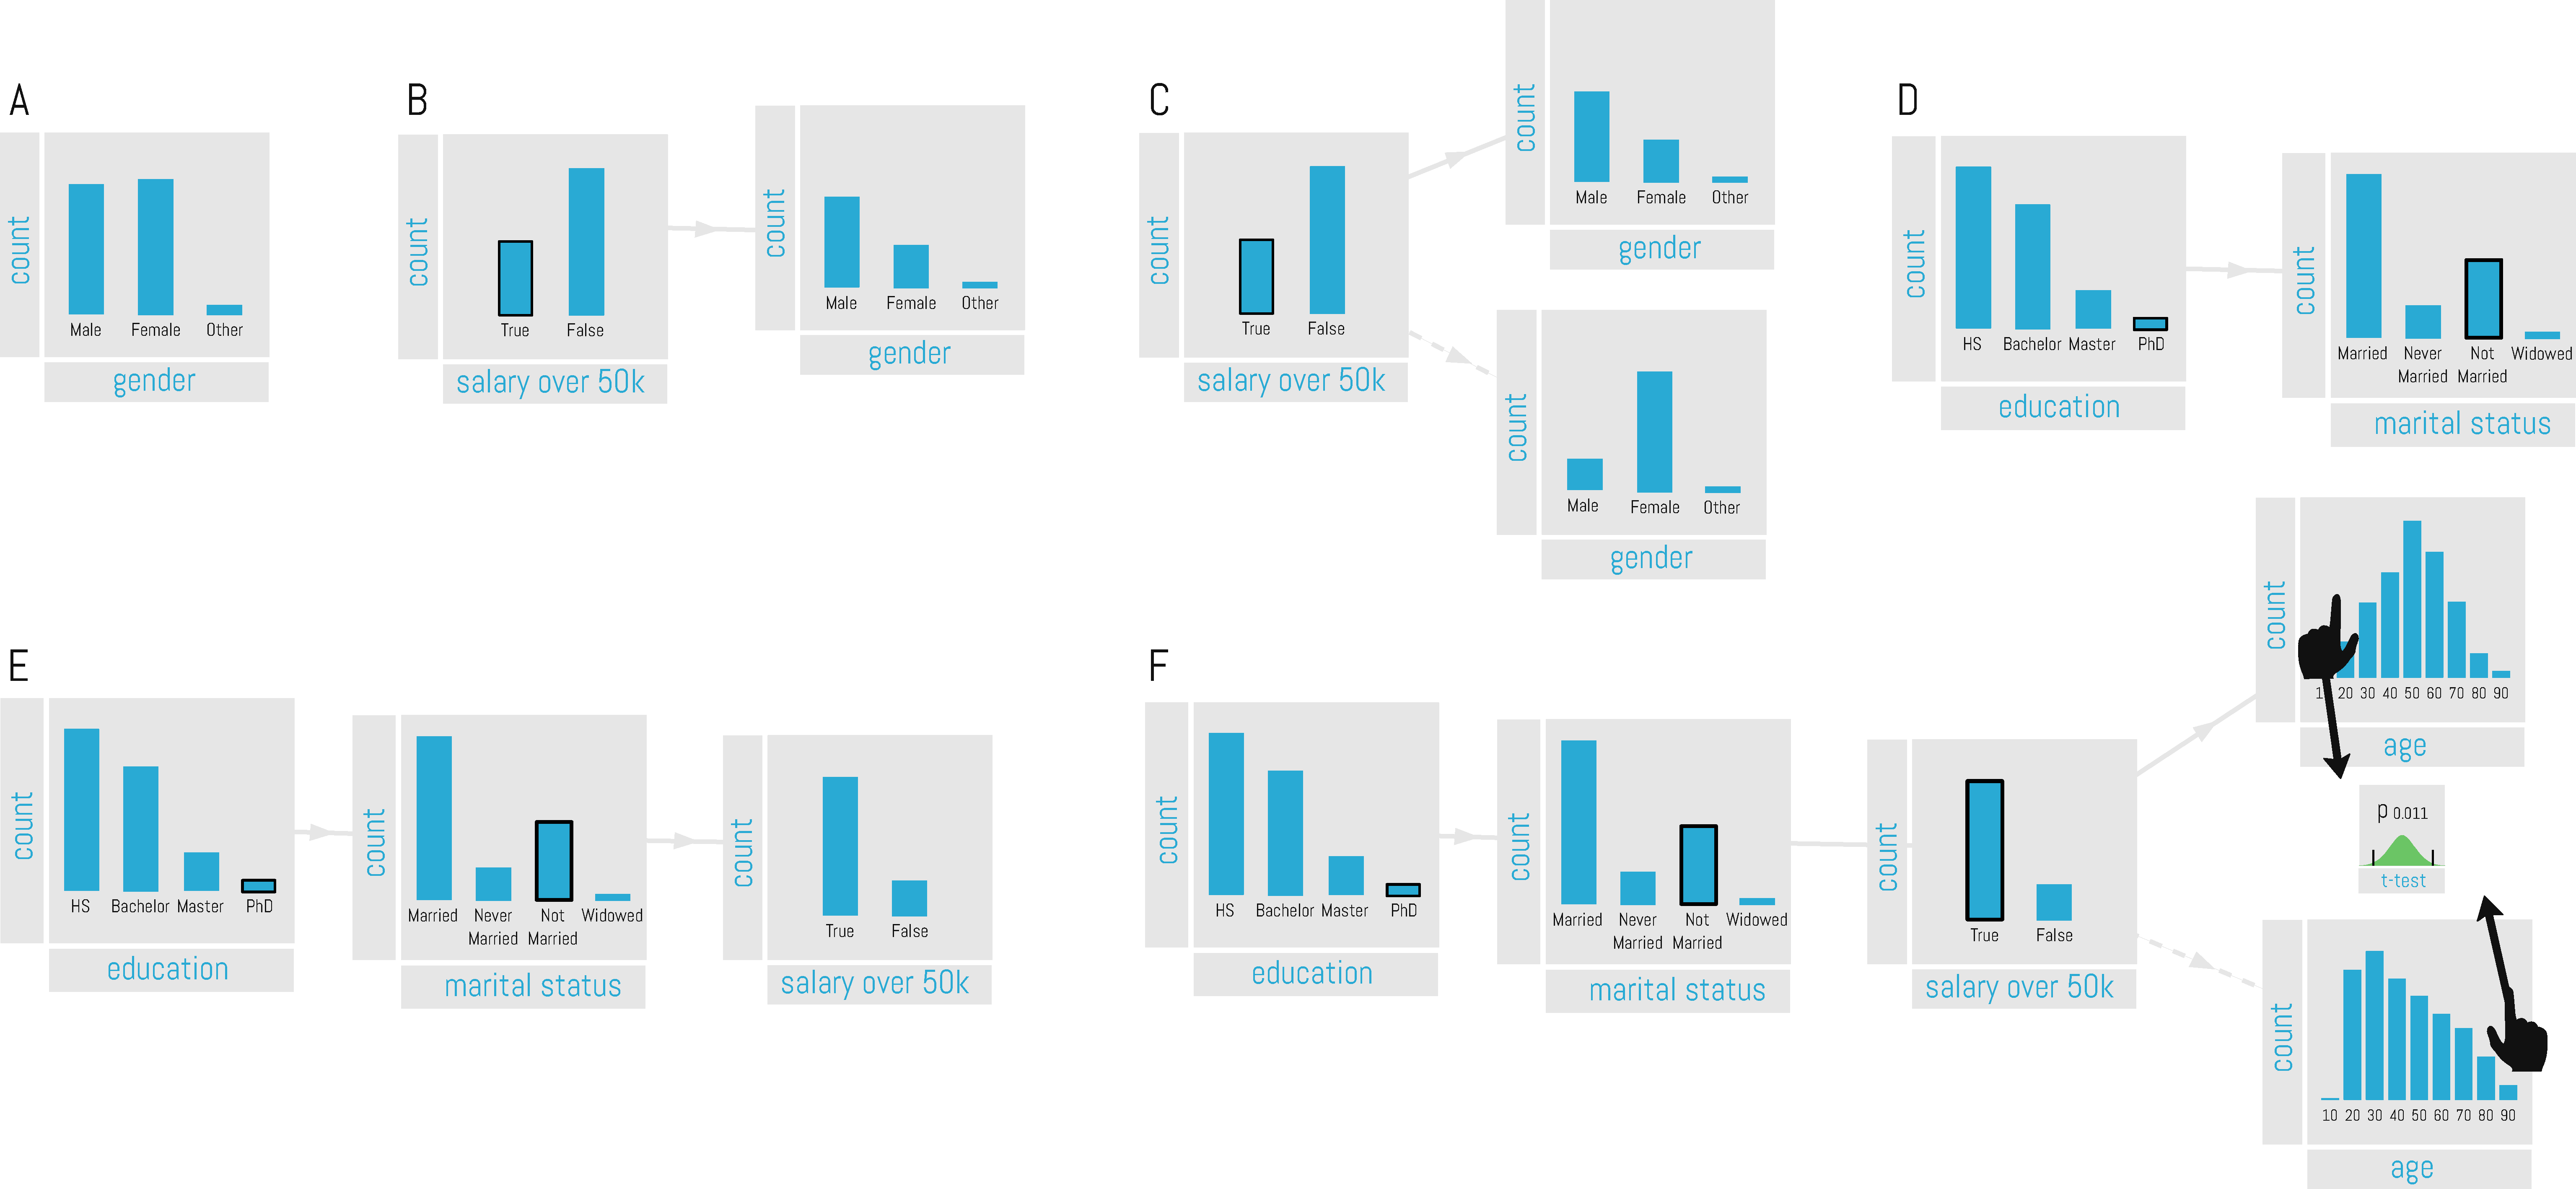
\includegraphics[width=0.9\textwidth]{figures/storyboard}
\end{center}\vspace{-5.5ex}
\vspace{-2.5ex}
\caption{An example Interactive Data Exploration Session}
\vspace{-3.5ex}
\label{fig:sb}	
\end{figure*}

\subsection{Visualizations as Hypotheses}
A visualization per-se shows a descriptive statistic (e.g., the count of women or the count of men) of the dataset and is not a hypothesis. 
It is reasonable to assume that in step~A of Figure~\ref{fig:sb} the user just looks at the gender distribution and simply acknowledges that the census surveys roughly the same amount of women and men.
However, it becomes an hypothesis test, if the user expected something else and draws a conclusion/inference based on the visualization. 
For example, if the user somehow assumed that there should be more men than women in the data and therefore considering the fact that there is an equal amount as an insight.
The notion of a visualization being considered as a hypothesis becomes even clearer in step~(B) and (C) of the example work-flow.
When looking at the visualization in (B) in isolation, it just depicts a descriptive statistic. 
Indeed, if the user would just take it as such and not make any inference about it and/or base further exploration on an insight extracted from this visualisation, then it would not be considered an hypothesis.
We argue however that the opposite is true more often than not. First, our analytical reasoning and sense-making process is inherently non-linear \cite{pirolli2005sensemaking,shrinivasan2008supporting}.
Our future actions are influenced by new knowledge we discovered in previous observations.
Second, while susceptible to certain types of biases \cite{attractionBias}, the human visual system is highly optimized at picking up differences in visual signals and at detecting patterns \cite{burgess1981efficiency}. 
An average user is very likely drawn to the changes between the gender distribution of step (A) and step (B) and might therefore infer that women earn less than men and potentially flag this as an interesting insight that deserves more investigation.
This is illustrated in step~(C) where the user now further drills down and visually compares the distribution of gender filtered by salary. 
We qualitatively confirmed this notion through a formative user study where we manually coded user-reported insights, following a think-aloud protocol similar to the one proposed in ~\cite{guo2016case}. In this study we observed that users tend to pick up on even slight differences in visualizations and regard them as insights and users predominantly base future exploration paths on previously inferred insights. 

We conclude two things: (1) most of the time users indeed treat visualizations as hypotheses, though there are exceptions, and (2) they often (wrongly) assume that what they see is statistical significant. 
The latter is particularly true if the users do not carefully check the axis on the actual count.  
For example, if a user starts to analyze the outliers of a billion record dataset and makes the conclusion that mainly uneducated whites are causing the outliers, the dataset she is referring to might be comparable small and the chance of randomness might be much higher. 
The same argument also holds against the critic, that with enough data observing differences by chance are much less likely, which is true. 
As part of visual data exploration tools, users often explore sub-populations, and while the original dataset might be large, the sub-population might be small. 
Thus, we argue that every visualization as part of a interactive data exploration tool should be treated as a hypothesis and that users should be informed about the significance of the insights they gain from the visualization. 
At the same time, a user should have the choice to declare a visualization as just descriptive. 

%\ez{i don't know this ref so not sure where to appropriately fit it in. - This effect is not new and lead for example to areas like visual data mining \cite{visualdatamining}}

\subsection{Heuristics for Visualization Hypotheses}
A core question remains: what should the hypothesis for a visualization be. 
Ideally, users would tell the system every single time what they are thinking so that the hypothesis is adjusted based on their assumed insight(s) they gain from the visualization. 
However, this is disruptive to any interactive data exploration session. 
We rather argue that the system should use a good default hypothesis, the user can modify (or even delete) if she so desires. 
For the purpose of this work, we mainly focus on histograms as shown in Figure~\ref{fig:sb} and acknowledge that there exist many other visualizations, which we consider as future work. 
We derived the following heuristics from two separate user studies where we observed over 50 participants using a IDE tool to explore various datasets. 

\vspace{-1.75ex}
\begin{enumerate*}
    \item {\em Every visualization without any filter conditions is not a hypothesis (e.g., step~A in Figure~\ref{fig:sb}) unless the user makes it one. } This is reasonable, as users usually first gain a general high-level impression of the data. Furthermore, in order to make it an hypothesis, the user would need to provide some prior knowledge/expectation, for example as discussed before, that he expected more men than women in the dataset. 
    \item {\em Every visualization with a filter condition is a hypothesis with the null-hypothesis that the filter condition makes no difference compared to the distribution of the whole dataset}. For example, in step~B of Figure~\ref{fig:sb} the null hypothesis for the distribution of men vs. women given the high salary class of over $\$50k$ would be that there is no difference compared to the equal distribution of men vs. women over the entire dataset (the visualization in step~A). This is again a reasonable assumption as the distribution of an attribute given others is only interesting, if it shows some different effect compared to looking at the whole dataset. 
    \item {\em If two visualization with the same but some negated filter conditions are put next to each other, it is a test with the null-hypothesis that there is no difference between the two visualized distributions, which supersedes the previous hypothesis.} This is the case in step~C: given that the user looks explicitly at the distribution of males vs females given a salary over and under $\$50k$ is a strong hint from the user, that he wants to compare these two distributions. 
\end{enumerate*}
\vspace{-2.0ex}

As with every heuristic it is important to note, that the heuristic can be wrong. 
Therefore it is extremely important to allow the user to overwrite the default hypothesis as well as delete default hypothesis if one really just acted as a descriptive statistic or was just generated as part to a bigger hypothesis test. 
Furthermore, there exist of course other potential null-hypothesis.
For example, in our workflow we assume by default that the user aims to compare distributions, which requires a  $\chi^2$-test.
However, maybe in some scenarios comparing the means (i.e., a t-test) might be more appropriate as the default test. Yet, studying in detail what a good default null-hypothesis is dependent on the data properties and domain, is beyond the scope of this paper. 

\subsection{Heuristics Applied to the Example}
For our example in Figure~\ref{fig:sb} the resulting hypothesis could be as follows:
Step~A is not an hypothesis based on rule 1 as it just visualizes the distribution of a single attribute over the whole dataset. 
Step~B is the hypothesis $m_1$ if the distribution of gender is different given a salary over $\$50k$. 
Step~C supersedes the previous hypothesis and replaces it with an hypothesis $m_1'$ if the gender distribution between a salary over and under $\$50k$ is different, which is a sightly different question. 
Step~D creates a hypothesis $m_2$ if the marital status for people with PhDs is different compared to the entire dataset, whereas step-E generates a hypothesis $m_3$ if there is a different salary distribution given not married people with a PhD. 
By studying the age distribution in step~F the system first generated a default hypothesis $m_4$  that the distribution of the ages is different given a PhD and being not married for different salary classes. 
However, the user overwrites immediately the default hypothesis with an hypothesis $m_4'$  about the average age. 
Furthermore, as the previous visualizations in step~D and E might just have been stepping stones towards creating $m_4‘$ the user might or might not delete hypothesis $m_2$ and $m_3$. 
However, if the insights our user gained from viewing the marital status, etc., influenced her to look at the age distribution, she might want to keep them as hypothesis. 

Clearly this is only a very small example, but it already demonstrates the general issues. 
Not every insight the user gains (e.g., the insight that women earn less) is explicitly expressed as a test. 
At the same time, as more the user ``surfs'' around the higher the chance that she finds something which looks interesting, but just appears because of chance. 
In the example above, by the time the user actually performs its first test (step~F), she implicitly already tested at least one other hypothesis and potentially even four others. 
Assuming a targeted \pval of $\alpha = 0.05$, the chance of a false discovery therefore increased to $1 - (1 - \alpha)^2=0.098$ for two hypothesis and up to $1 - (1 - \alpha)^4=0.185$ for four hypothesis. 
While the question of what should count as an hypothesis is highly dependent on the user and can never be fully controlled by any system, we can however, enable the system to make good suggestions and help users to track the risk of making false discoveries by chance. 
Furthermore, this short workflow also demonstrates that hypotheses are built by adding but also by removing attributes. 
As we will discuss later, there exist no good method so far to control the risk of making false discoveries for incremental sessions like the ones created by interactive data exploration systems. 
We therefore develop new methods especially for interactive data exploration in Section~\ref{sec:invest}.
%Finally, the situation gets even worse with automatic visualization recommendation engines or correlation finders, as \cite{cidrrisk} already pointed out. 
%While ``safe'' recommendations are beyond the scope of this paper, we will outline potential initial solutions in Section~\ref{sec:fdrcontrol}.

Finally, it should be noted, that the same problems also exist with exploratory analysis using SQL or other tools. 
However, we argue that the situation is becoming worse by the up-rise of visual exploration tools, like Tableau, which are often used by novice users, who not necessarily reflect enough on their exploration path after they found something interesting. 




%In the following section we outlined the challenges associated with automatic risk control. 
%We therefore describe first a common data exploration session and afterwards derive from it the common challenges. 


%- Incremental
%- Chains
%- Backtracking
%- Select most important hypothesis 
%- Default Hypothesis
%- sustainable recommendations. 

%Say something about old SQL